        \clearpage
        \begin{figure*}[ht]
            \pdfbookmark[2]{ID 01}{figure_id_01}
        	\centering
            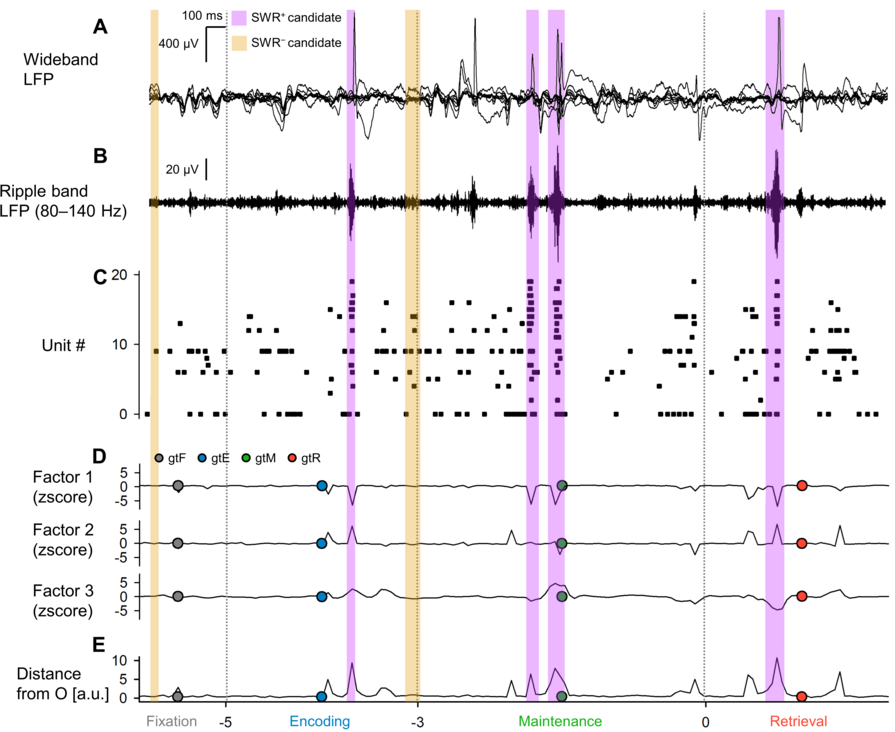
\includegraphics[width=1\textwidth]{./src/figures/.png/Figure_ID_01.png}
        	\caption{\textbf{
Local Field Potentials, Multiunit Activity, and Neural Trajectories in the Hippocampus during a Modified Sternberg Task
}
\smallskip
\\
\textbf{\textit{A.}} Presented are representative wideband LFP signals for an intracranial EEG recording from the left hippocampal head, obtained while the subject performed a modified Sternberg working memory task. The task comprises stages of fixation (1s, \textit{gray}), encoding (2s, \textit{blue}), maintenance (3s, \textit{green}), and retrieval (2s, \textit{red}). \textbf{\textit{B.}} Depicted are the associated ripple band LFP traces. Pay attention to the \textit{purple} and \textit{yellow} rectangles, which represent the timings for SWR$^+$ candidates and SWR$^-$ candidates, respectively (the latter serve as control events for SWR$^+$). \textbf{\textit{C.}} A raster plot demonstrates multi-unit spikes obtained from the LFP traces, sorted using a spike algorithm \cite{niediek_reliable_2016}. \textbf{\textit{D.}} The neural trajectories (NTs) calculated by GPFA\cite{yu_gaussian-process_2009} based on spike counts per unit with 50-ms bins are displayed; the geometric median of each phase is marked by dot circles. \textbf{\textit{E.}} The distance of the NT from the origin point $O$ is shown.
}
% width=1\textwidth
        	\label{fig:01}
        \end{figure*}
